\documentclass{article}
\usepackage[top=1in, bottom=1in, left=1in, right=1in]{geometry}
\usepackage{amsfonts, amsmath, amssymb, amsthm}
\usepackage{mathtools}
\usepackage{enumerate}
\usepackage{enumitem}
\usepackage{fancyhdr}
\usepackage{listings}
\usepackage{array}
\usepackage{float}
\usepackage{changepage}
\usepackage{longtable}
\usepackage{dirtree}
\usepackage[export]{adjustbox}

\lstset{basicstyle=\ttfamily, breaklines=false}
\setlength{\DTbaselineskip}{15pt}
\DTsetlength{1em}{5em}{0.5em}{1pt}{1.8pt}
\renewcommand*\DTstyle{\large\ttfamily}
\newcolumntype{L}[1]{>{\raggedright\let\newline\\\arraybackslash\hspace{0pt}}m{#1}}
\newcolumntype{C}[1]{>{\centering\let\newline\\\arraybackslash\hspace{0pt}}m{#1}}
\newcolumntype{R}[1]{>{\raggedleft\let\newline\\\arraybackslash\hspace{0pt}}m{#1}}

\pagestyle{fancy}
\fancyhead[L]{CSE 141L, Computer Architecture}
\fancyhead[R]{Lab2, Verilog Modules}
\setlength{\headheight}{26pt}
\setlength{\headsep}{16pt}

\title{\quad
  \\ [4.0cm]
  \normalsize \textsc{CSE 141L \\ Spring, 2017}
  \\ [2.0cm]
  \huge \textbf{\uppercase{Verilog Modules}}
  \\ [0.5cm]
  \normalsize \today}
\author{}
\date{}
\begin{document}
  \maketitle
  \vspace{6.0cm}
  \begin{large}
    \begin{center}
      \begin{tabular}{l r}
        Author:        & Chenxu Jiang \\
        PID:            & A92114155 \\
        Author:        & Dingcheng Hu \\
        PID:            & A92090168
      \end{tabular}
    \end{center}
  \end{large}
  \newpage
  \section{Introduction}
    In this lab, we build verilog modules for our CPU, in logic level.
    We build the following modules:
    \begin{description}
      \item[ALU] supports addition/subtraction, 1-bit shifting, and branching
        decision.
      \item[Register File] contains 3 sub-module, Accumulator Register
        Regular Register and Single-Bit Register.
      \item[Data Memory] is 256 in depth and 8-bit in width, supports
        reads and writing to an memory address.
      \item[Instruction Fetch] that contains Program Counter (its increment,
        branching and halting logic), Instruction Memory that stores read-only
        intruction memory and Look-up Table that stores branching address.
    \end{description}
  \section{ISA Summarization}
    There are following types of operations supported:
    \begin{description}
      \item[Data Type:] \quad \\
        Load from Memory Address to Register \\
        Store from Register to Memory Address. \\
        Copy Data in one Register to another Register.
      \item[Arithmetic Type:] \quad \\
        Addition/Subtration of 2 Registers with/without Stored Overflow Bit. \\
        Right Shifting Logically/Arithmetically/use stored Overflow Bit as shift-in. \\
        Left Shifting that always use Overflow Bit as shift-in.
      \item[Miscellaneous:] \quad \\
        Zero Specified Register. \\
        Decrementing Specified Register by 1. \\
        Add one Register 1 to Register 2 only if Register 3 is not negative. \\
        Flip stored Flip-bit if specified register is negative. \\
        Add 1 to Register 1 if the upper-4-bit of Register 2 and 3 matches. \\
        Add flip bit xor flag bit to specified register.
      \item[Branching:] \quad \\
        Branch if specified register is not 0. \\
        Branch if upper-4-bit of specified register is not 0. \\
        Branch if the register not equal to 31.
    \end{description}
  \section{ALU Operations}
    ALU need to support all Arithmetic Type, Miscellaneous and Branching Instruction.
    \begin{description}
      \item[Arithmetic Type:] \quad \\
        Addition/Subtration of 2 Registers with/without Stored Overflow Bit. \\
        \text{\quad -} \texttt{add1, add4, add5, addf0, addf4, sub1, sub3, sub4, sub5, subf2, sub25, add25, subf25} \\
        Right Shifting Logically/Arithmetically/use stored Overflow Bit as shift-in. \\
        \text{\quad -} \texttt{srl, sra, srf, srl4, sra5, srf5} \\
        Left Shifting that always use Overflow Bit as shift-in. \\
        \text{\quad -} \texttt{slf0, slf1, slf2}
      \item[Miscellaneous:] \quad \\
        Zero Specified Register. \\
        \text{\quad -} \texttt{zero0, zero2, zero3, zero4} \\
        Decrementing Specified Register by 1. \\
        \text{\quad -} \texttt{dec1} \\
        Add one Register 1 to Register 2 only if Register 3 is not negative. \\
        \text{\quad -} \texttt{add3\_n2, add4\_n2} \\
        Flip stored Flip-bit if specified register is negative. \\
        \text{\quad -} \texttt{atos\_2} \\
        Add 1 to Register 1 if the upper-4-bit of Register 2 and 3 matches. \\
        \text{\quad -} \texttt{add0c25} \\
        Add flip bit xor flag bit to specified register.
        \text{\quad -} \texttt{inc\_af0}
      \item[Branching:] \quad \\
        Branch if specified register is not 0. \\
        \text{\quad -} \texttt{bnzr} \\
        Branch if upper-4-bit of specified register is not 0. \\
        \text{\quad -} \texttt{bnuzr} \\
        Branch if the register not equal to 31. \\
        \text{\quad -} \texttt{b1ne31}
    \end{description}
  \section{Verilog Modules}
    \subsection{Hierarchy Tree}
      \dirtree{%
        .1 SingleCycleCPU.sv.
        .2 ALU.sv.
        .3 Adder.sv.
        .3 Shifter.sv.
        .2 InstrDecode.sv.
        .2 InstrFetch.sv.
        .3 InstrMem.sv.
        .3 LookupTable.sv.
        .3 ProgramCounter.sv.
        .2 RegsFile.sv.
        .3 AccumulatorRegs.sv.
        .3 RegularRegs.sv.
        .3 SingleBitRegs.sv.
        .2 DataMem.sv.
      }
    \newpage
    \subsection{Schematics}
    \begin{figure}[h]
      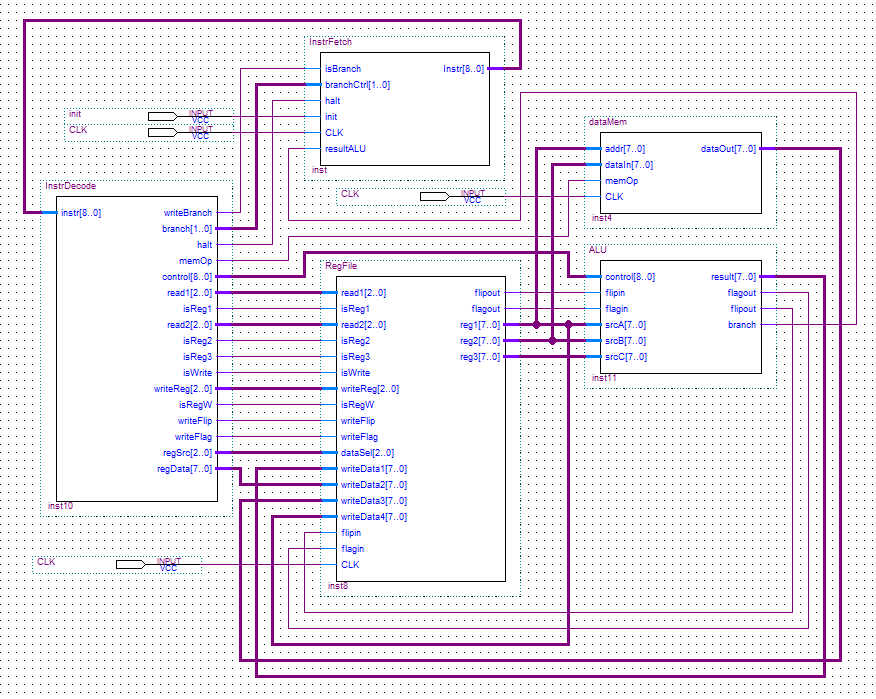
\includegraphics[width=\textwidth]{schematics.png}
    \end{figure}
  \newpage
  \section{Time Diagram}
    \subsection{ALU Test}
    \vspace{-15mm}
    \begin{figure}[H]
      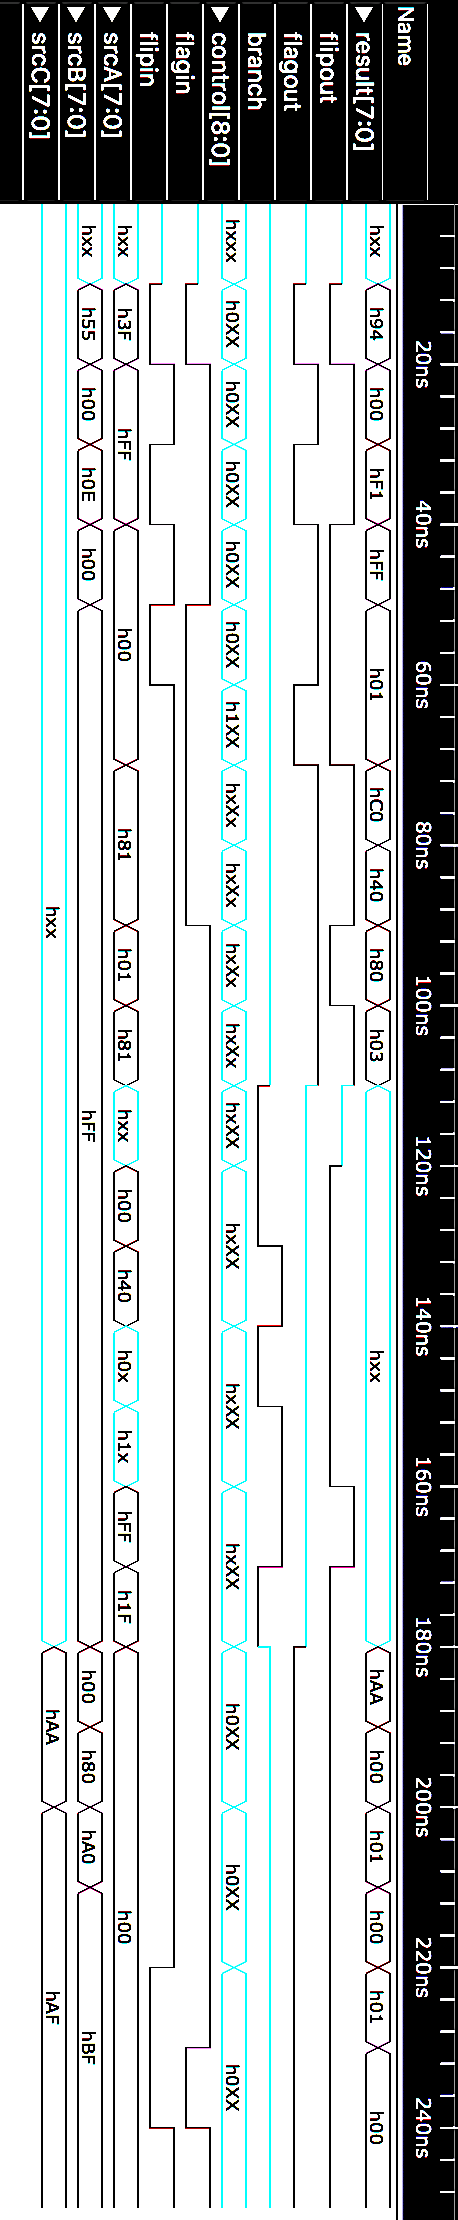
\includegraphics[width=0.293\textwidth, right]{ALUTest.png}
    \end{figure}
    \newpage
    \subsection{Register File Test}
    \vspace{-10mm}
    \begin{figure}[H]
      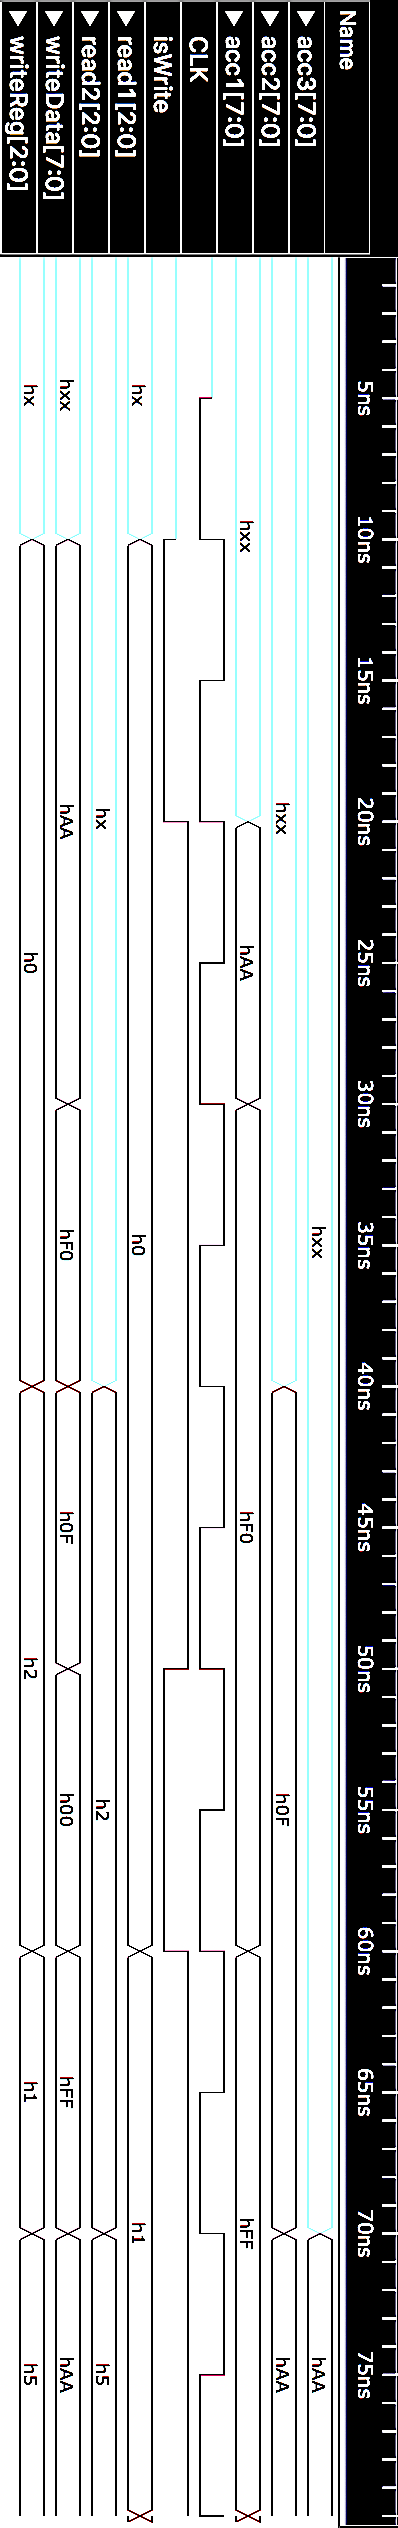
\includegraphics[width=0.224\textwidth, right]{RegTest.png}
    \end{figure}
    \newpage
    \subsection{Instruction Fetch Test}
    \vspace{-10mm}
    \begin{figure}[H]
      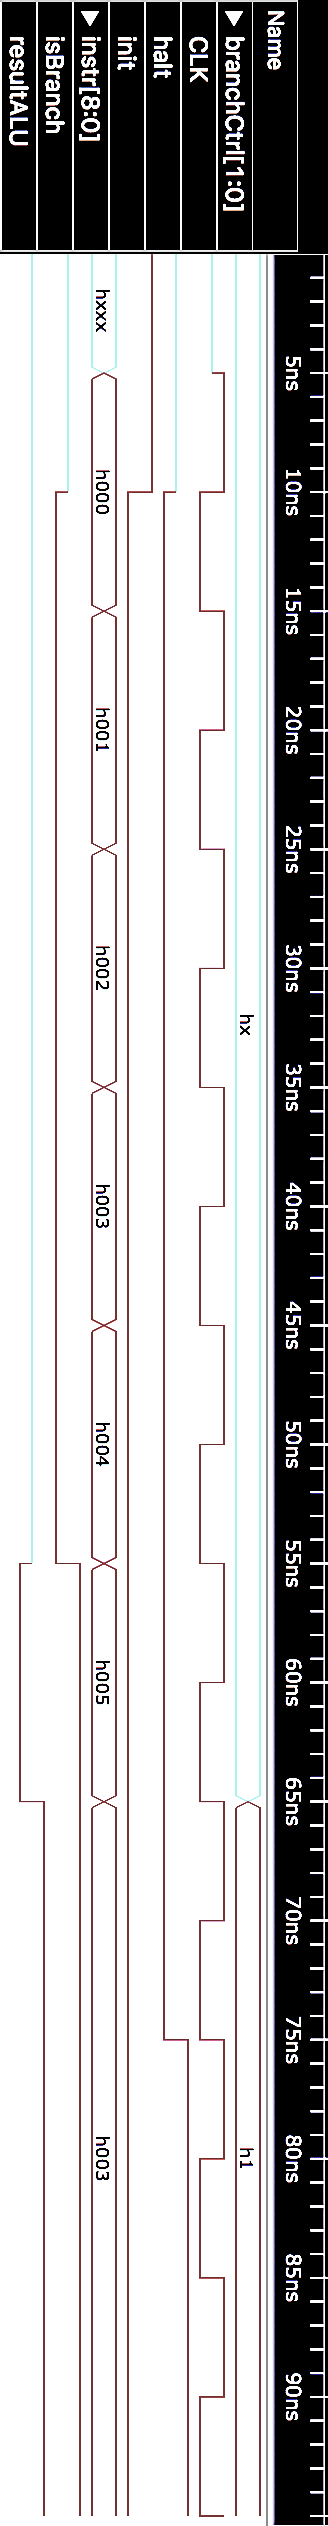
\includegraphics[width=0.185\textwidth, right]{IFTest.png}
    \end{figure}
    \newpage
  \section{Non-Arithmetic Instruction in ALU}
    \quad We use ALU for determining branching. We use 3 branching
    and the determination is paralleled with adder and shifter.
    Therefore, for time's sake there is no difference. But more
    gates are used to judge if branch or not.
  \section{Easier Instruction Fetch}
    \quad We think our Instruction Fetch is already easy enough.
    It can be made without branching address stored in lookup table.
    But without lookup table the branching distance would limited
    to only +/- 8 instructions, which is not enough.
  \section{Easier ALU Design}
    \quad Our ALU does too much jobs, since there are lots of
    instruction specifically made up for the 3 program, to reduce
    instruction count. If we don't need to reduce Instruction
    count, then the logic in ALU can be limited to adder and
    shifter, and become easier.
  \section{Easier Register File}
    \quad Our register file is very complicated, since we divide
    it into 2 parts, Accumulator Registers and Regular Registers.
    It is divided, since we have only 9-bit instruction and we
    manage to give register 2-bit. Therefore, we came to the idea
    of dividing register. Regular register can be use as argument.
    and accumulator register can be used as accumulator, and is
    included in the instruction name. Division of register file
    is like put a mux manually between the 2 register files. If we
    have more bits for instruction code, then we will not need
    the division. And our register file can be easier.
  \section{Most Complex Instruction ALU}
    \quad \texttt{add3\_n2, add4\_n2, add0c25, inc\_af0} are 4 most
    complex instructions for ALU. They are the only 4 instructions
    that need ALU to preprocess the input to adder. The other
    instructions have value directly go to adder or shifter.
  \section{Additional Function of ALU}
    No. The design can only execute instruction that it is made for.
\end{document}
